\chapter{Multi-task learning}

So far we have considered \ac{AES} and \ac{NLI} as independent tasks and
performed experiments on both tasks separately. We will now try to train
models to predict both tasks simultaneously.


\section{Models}

We selected four models for the multi-task experiments, two convolutional and
two recurrent neural networks. They were chosen based on the macro \FI results
on the development set. The two \acp{CNN} chosen were the two \acp{CNN} that
had the highest macro \FI on the full set of labels in the development set,
and likewise for the two \acp{RNN}. The hyperparameters for the four models are
summarized in tables \ref{tab:cnn-parameters} and \ref{tab:rnn-parameters}.

\begin{table}
  \centering
  \begin{tabular}{lll}
    \toprule
    Hyperparameter & CNN1 & CNN2 \\
    \midrule
    Word embeddings & \multicolumn{2}{c}{Dynamic} \\
    Embedding size & \multicolumn{2}{c}{100} \\
    $L_2$ constraint & \multicolumn{2}{c}{3} \\
    Windows & \multicolumn{2}{c}{3,4,5} \\
    Embedding init & Random & Pre-trained \\
    Input representation & Mixed UPOS & Tokens \\
    \bottomrule
  \end{tabular}
  \caption{Descriptions of the two CNN models}
  \label{tab:cnn-parameters}
\end{table}

\begin{table}
  \centering
  \begin{tabular}{lll}
    \toprule
    Hyperparameter & RNN1 & RNN2 \\
    \midrule
    Word embeddings & \multicolumn{2}{c}{Dynamic} \\
    Embedding size & \multicolumn{2}{c}{100} \\
    RNN cell & \multicolumn{2}{c}{GRU} \\
    Pooling method & \multicolumn{2}{c}{Attention} \\
    Bidirectional & \multicolumn{2}{c}{Yes} \\
    Embedding init & Random & Pre-trained \\
    Input representation & Tokens+UPOS & Tokens \\
    \bottomrule
  \end{tabular}
  \caption{Descriptions of the two RNN models}
  \label{tab:rnn-parameters}
\end{table}

The multi-task models have two outputs with different loss functions. The
CEFR output is a single regression node with sigmoid output and mean squared
error loss. The NLI output is a softmax layer with seven nodes, and uses
categorical cross-entropy loss. To train the models, they are optimized to
minimize the sum of losses for both output layers. We multiply each loss by a
weight before summing to see how performance is influenced by which loss has
most weight. We ensure that the sum of weights is equal to 1. An auxiliary
loss weight of $0.5$ thus means that both losses have equal weight. An
auxiliary loss weight of $0.2$ means that the loss on the main task has
weight $0.8$.

We chose ten different auxiliary loss weights, and for each loss weight we
trained and evaluated each model five times with different random seeds. By
training more than one model with a given set of hyperparameters, we can get
an idea of the variance of results.

\section{Results}

Below we plot see the results of running some of the most successful models
from the previous chapter in a multi-task setting, using the essay's L1 as
the auxiliary label to predict. The $x$ value is the weight given to the
auxiliary loss during training. Some of the models have an auxiliary loss
weight of zero, which is the same as training in single-task mode.

\todo{outdated}
The reported metrics apply to the main task, CEFR prediction, only. It seems
that the auxiliary task is beneficial for all CNN models. All CNN models get
higher macro and micro \FI in the multi-task setup. Moreover, a higher weight
given to the auxiliary L1 prediction task seems to improve macro \FI
performance across the board. The effect of the auxiliary task weight seems
less clear on the micro \FI. but remember that in our setup, the micro \FI is
a side effect of the highest macro \FI seen during training.

\begin{figure}
  \centering
  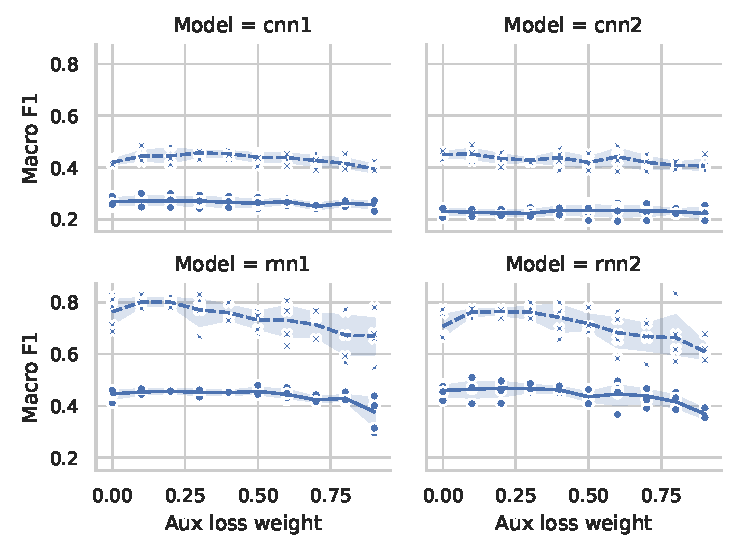
\includegraphics{lossweight}
  \caption[Performance of multi-task models]{
    Lines follow the mean of macro \FI scores. Shaded areas show 95\% confidence
    interval for the mean. Results for the collapsed set of classes are plotted with
    cross symbols and dashed lines.
  }
  \label{fig:lossweight}
\end{figure}

\todo{must check again}
The highest macro \FI scores on the full label set all come from the RNN2 model.
The five highest scores range between $0.486$ and $0.509$ and were achieved
using auxiliary loss weights in the range from $0.1$ to $0.6$.

\todo{outdated}
The model `RNN1 0.5' was the best performing multi-task model by several
metrics. In addition to macro \FI, it was the best in terms of RMSE
($0.888$), MAE ($0.610$), Pearson's correlation coefficient ($0.765$) and
Spearman's ranked correlation coefficient ($0.768$).


\begin{figure}
  % cnn-multi-26199963_11
  \begin{subfigure}{\linewidth}
    \centering
    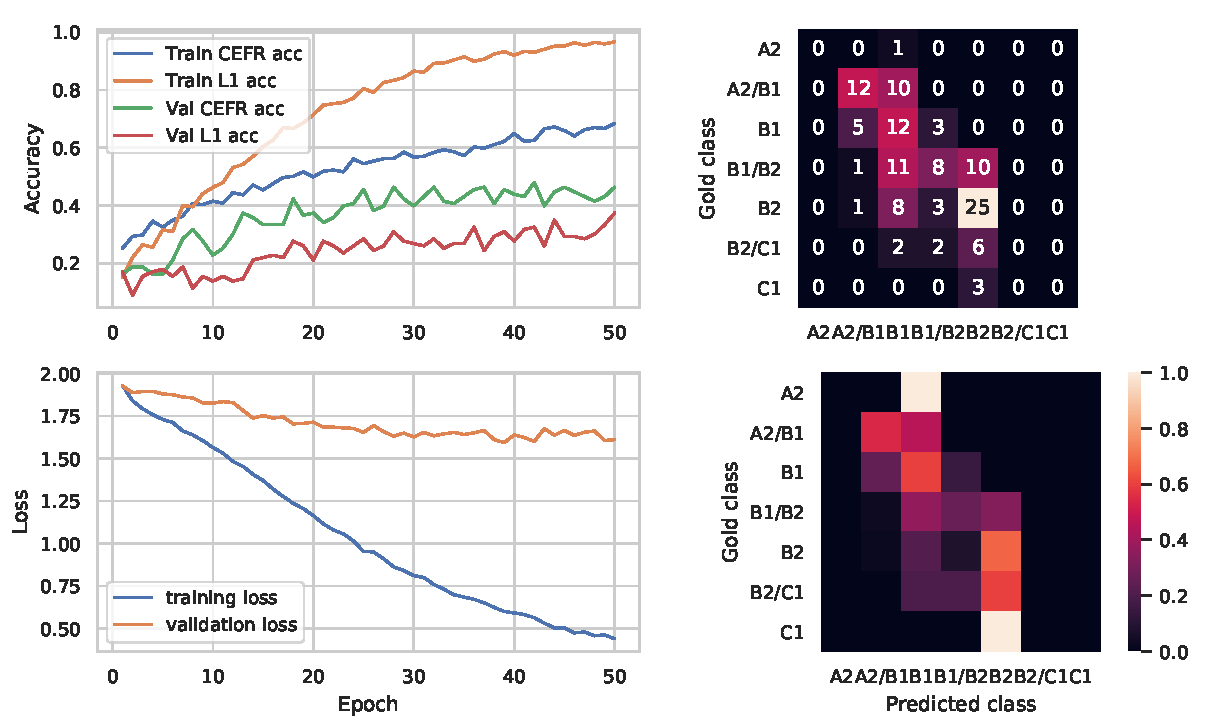
\includegraphics{cnn-multi-training}
    \caption{Training and validation loss and accuracy over 50 epochs of training.}
  \end{subfigure}
  \begin{subfigure}{\linewidth}
    \centering
    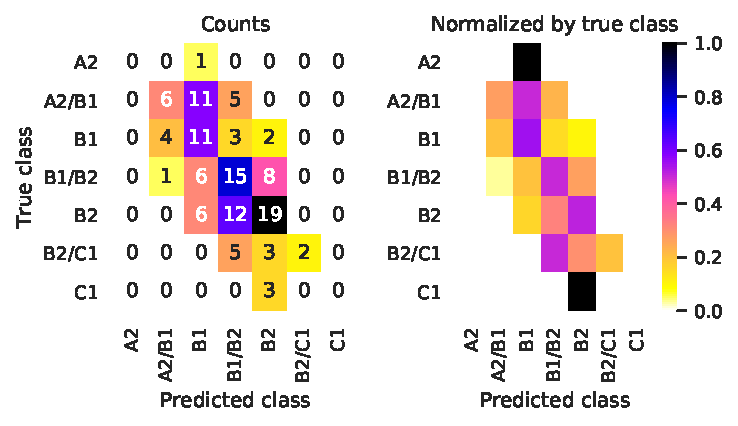
\includegraphics{cnn-multi-confusion}
    \caption{Confusion matrix on validation set, raw counts and normalized.}
  \end{subfigure}
  \caption{CNN2 0.75}
  \label{fig:cnn-multi-training}
\end{figure}

\begin{figure}
  % rnn-multi-26646843_28.pkl
  \begin{subfigure}{\linewidth}
    \centering
    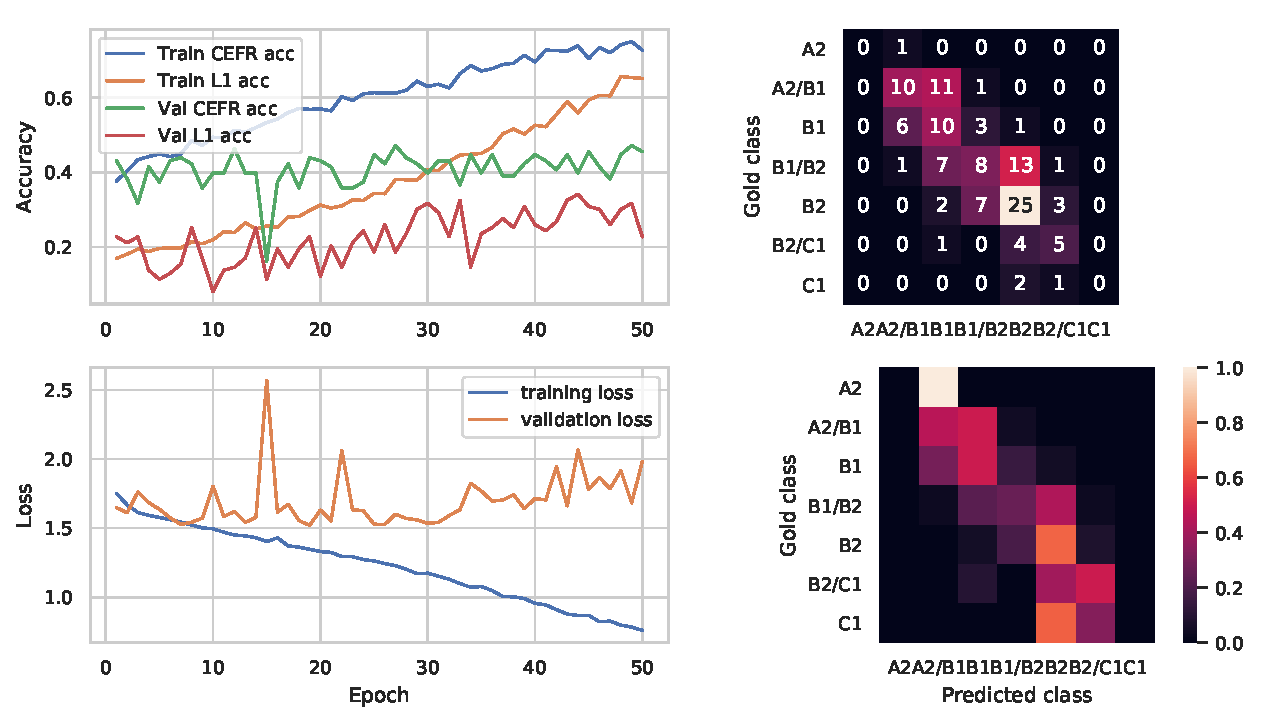
\includegraphics{rnn-multi-training}
    \caption{Training and validation loss and accuracy over 50 epochs of training.}
  \end{subfigure}
  \begin{subfigure}{\linewidth}
    \centering
    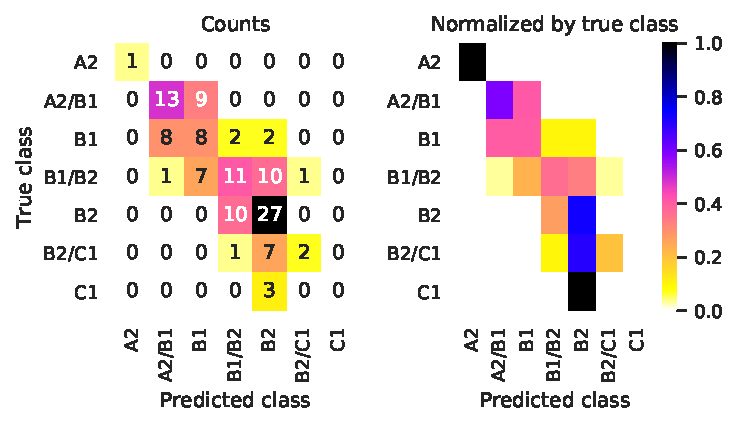
\includegraphics{rnn-multi-confusion}
    \caption{Confusion matrix on validation set, raw counts and normalized.}
  \end{subfigure}
  \caption{RNN1 0.5}
  \label{fig:rnn-multi-training}
\end{figure}


\section{Correlation of metrics}

\todo{More different metrics}

We have previously discussed different evaluation metrics. Since we now have
trained and evaluated a number of different models, it is possible to see
whether the metrics agree on the ranking of models.

Macro \FI and macro \ac{MAE} correlates only weakly, as seen in figure
\ref{fig:f1-vs-mae}, but they seem to agree on the highest ranking models:
The Pareto front consists of only two samples. The samples in the plot are
models that predict the full seven classes.

\begin{figure}
  \centering
  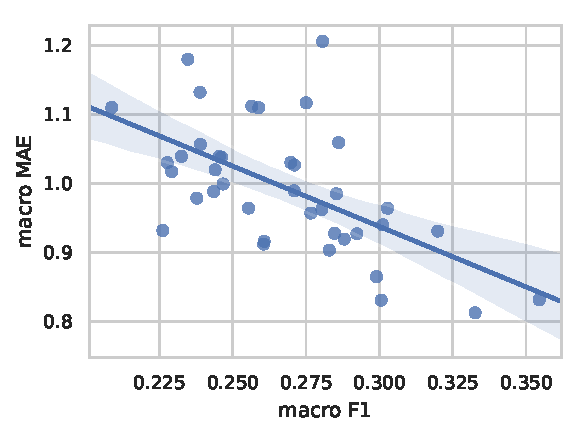
\includegraphics{f1-vs-mae}
  \caption[Macro \FI versus macro MAE]{
    Macro \FI versus macro MAE. Pearson's correlation coefficient = $-0.5945$,
    $p < 10^{-4}$. The shaded area covers a 95\% confidence interval for the
    line of regression.
  }
  \label{fig:f1-vs-mae}
\end{figure}
